\pdfoutput=1
\documentclass{article} % For LaTeX2e
\usepackage{iclr2017_workshop,times}
\usepackage{hyperref}
\usepackage{url}

% my imports
\usepackage{amssymb,amsmath,amsthm}
\usepackage[makeroom]{cancel}

\usepackage{algorithm}
\usepackage[noend]{algpseudocode}


\usepackage{graphicx}
\usepackage{multirow,bigstrut}
\newcommand{\eqname}[1]{\tag*{#1}}

\usepackage{textcomp}

\usepackage{bm}

% \usepackage{subcaption}
% \usepackage{float}
% \usepackage{array}
\usepackage{subfig} 
% \usepackage{tikz} 
% \usetikzlibrary{bayesnet}

%this is here just to remove some errors
\DeclareCaptionSubType*{algorithm}
\renewcommand\thesubalgorithm{\thetable\alph{subalgorithm}}


\definecolor{mydarkblue}{rgb}{0,0.08,0.45}
\definecolor{myfavblue}{rgb}{0.1176, 0.392, 1.0}
\hypersetup{
    colorlinks=true,
    linkcolor=mydarkblue,
    citecolor=mydarkblue,
    filecolor=mydarkblue,
    urlcolor=mydarkblue}






\title{Reinterpreting Importance-Weighted \\Autoencoders}


\author{Chris Cremer, Quaid Morris \& David Duvenaud \\
Department of Computer Science\\
University of Toronto\\
%Toronto, ON, Canada \\
\texttt{\{ccremer,duvenaud\}@cs.toronto.edu} \\
\texttt{\{quaid.morris\}@utoronto.ca}
% \texttt{ccremer@cs.toronto.edu},\texttt{quaid.morris@utoronto.ca},\texttt{duvenaud@cs.toronto.edu}\\
}

\newcommand{\fix}{\marginpar{FIX}}
\newcommand{\new}{\marginpar{NEW}}

\begin{document}


\maketitle

\begin{abstract}
The standard interpretation of importance-weighted autoencoders is that they maximize a tighter lower bound on the marginal likelihood than the standard evidence lower bound.
We give an alternate interpretation of this procedure: that it optimizes the standard variational lower bound, but using a more complex distribution. 
We formally derive this result, present a tighter lower bound, and visualize the implicit importance-weighted distribution.
%This distribution, $\tilde{q}_{IW}(z|x)$, is an importance weighted distribution implicitly defined by the  a pointwise reweighting of a parametric base distribution $q(z|x)$.
%We also propose a family of extensions allowing iterative refinement of the approximate posterior based on gradients of the log-likelihood.
\end{abstract}
 

\begin{figure}[b]
  \centering
   True posterior \qquad  \qquad $k=1$  \qquad \qquad \qquad $k=10$ \qquad \qquad \qquad $k=100$ \quad
      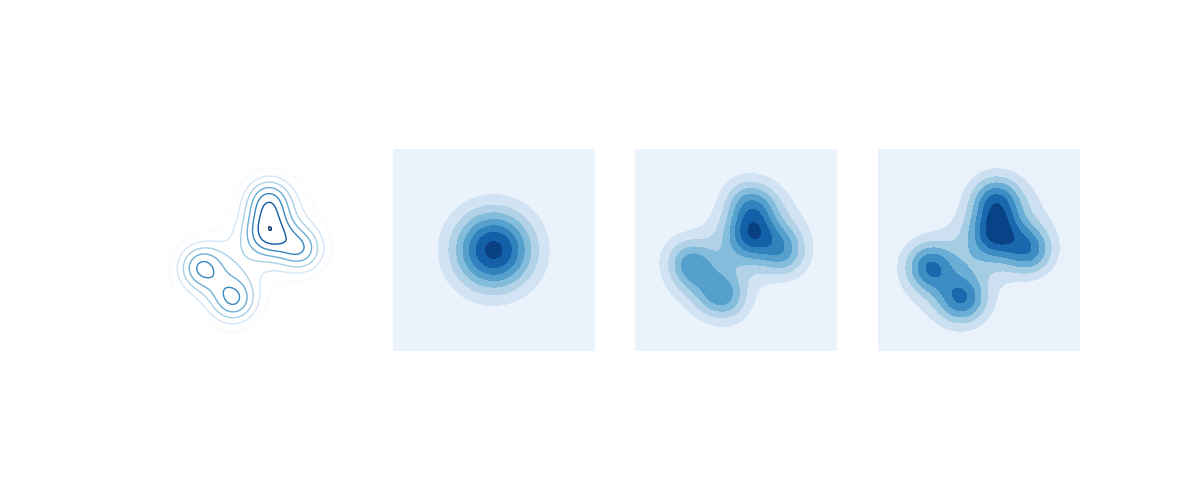
\includegraphics[width=1.\textwidth, clip, trim=2.5cm 3.9cm 2cm 3.6cm]{figs/figure_1.png}
  \vspace{-5mm}
  \caption{Approximations to a complex true distribution, defined via $q_{EIW}$.
%   sampling-importance-resampling. 
  As $k$ grows, this approximation approaches the true distribution.}
  \label{viz1}
\end{figure}


\section{Background}
The importance-weighted autoencoder (IWAE; \cite{burda2015importance}) is a variational inference strategy capable of producing arbitrarily tight evidence lower bounds. IWAE maximizes the following multi-sample evidence lower bound (ELBO): 
\begin{align} 
    \log p(x) &
    % log\left(E_{z_{1}...z_{k} \sim q(z|x)} \left[  \frac{1}{k}\sum_{i=1}^k \frac{p(x,z_i)}{q(z_i|x)}    \right]   \right)_{ML}
    % \\
    % & 
    \geq E_{z_{1}...z_{k} \sim q(z|x)} \left[\log\left(  \frac{1}{k}  \sum_{i=1}^k \frac{p(x,z_i)}{q(z_i|x)}  \right)  \right] = L_{IWAE}[q] \label{iwae_elbo}  \eqname{(IWAE ELBO)}
\end{align}
which is a tighter lower bound than the ELBO maximized by the variational autoencoder (VAE; \cite{vae}):
% \begin{align}
%     log(p(x)) & \geq E_{z_{1}...z_{k} \sim q(z|x)} \left[  \frac{1}{k}\sum_{i=1}^k \log\left(\frac{p(x,z_i)}{q(z_i|x)}  \right)  \right] = L_{VAE}[q]. \label{vae_elbo} \eqname{(VAE ELBO)}
% \end{align}
\begin{align}
    \log p(x) & \geq E_{z \sim q(z|x)} \left[ \log\left(\frac{p(x,z)}{q(z|x)}  \right)  \right] = L_{VAE}[q]. \label{vae_elbo} \eqname{(VAE ELBO)}
\end{align}
% Here we've written the VAE bound as a multisample lower bound to compare it to the IWAE bound. 


% %maybe put this in discussion, need to use reparam trick

% The following equations are the gradients of the VAE ELBO and the IWAE ELBO, respectively:
% \begin{align} 
%     \nabla_{\Theta} \mathcal{L}_{VAE}[q] &= E_{\epsilon_{1}...\epsilon_{k} \sim N(0,1)} \left[   \sum_{i=1}^k \frac{1}{k} \nabla_{\Theta} \log\left(\frac{p(x,z_i)}{q(z_i|x)}  \right)  \right] \label{vae_grad} \\
% % \end{align}
% % \begin{align} 
%     \nabla_{\Theta} \mathcal{L}_{IWAE}[q] &= E_{\epsilon_{1}...\epsilon_{k} \sim N(0,1)} \left[  \sum_{i=1}^k \tilde{w}_i \nabla_{\Theta} \log\left(\frac{p(x,z_i)}{q(z_i|x)}  \right)  \right] \label{iwae_grad}
% \end{align}
% where $$\tilde{w}_i = \frac{\frac{p(x,z_i)}{q(z_i|x)}}{\sum_{j=1}^k \frac{p(x,z_j)}{q(z_j|x)}}.$$

% From equations \eqref{vae_grad} and \eqref{iwae_grad}, we see that the gradient of the VAE ELBO evenly weights the samples, whereas the IWAE gradient weights the samples based on their relative importance $\tilde{w}_i$.






\section{Defining the implicit distribution \texorpdfstring{$\tilde{q}_{IW}$}{}}

%From the gradient of the IWAE bound (Eqn. \ref{iwae_grad}), we know that each sample is weighted by their importance $\tilde{w}_i$. This weighting implicitly defines a nonparametric approximate posterior.

In this section, we derive the implicit distribution that arises from importance sampling from a distribution $p$ using $q$ as a proposal distribution. Given a batch of samples $z_{2}...z_{k}$ from $q(z|x)$, the following is the unnormalized importance weighted distribution:
% \begin{align} 
%     \tilde{q}_{IW}(z|x,z_{2:k}) = k \tilde{w} q(z|x)
%     & = \left( \frac{ \frac{p(x,z)}{q(z|x)}}{  \frac{1}{k}   \sum_{j=1}^k \frac{p(x,z_j)}{q(z_j|x)}}  \right) q(z|x)
%     = \frac{p(x,z)}{\frac{1}{k} \left(  \frac{p(x,z)}{q(z|x)}+ \sum_{j=2}^k \frac{p(x,z_j)}{q(z_j|x)} \right)} 
% \label{eq:qiw}
% \end{align}
\begin{align} 
    \tilde{q}_{IW}(z|x,z_{2:k}) =  \frac{ \frac{p(x,z)}{q(z|x)}}{  \frac{1}{k}   \sum_{j=1}^k \frac{p(x,z_j)}{q(z_j|x)}}   q(z|x)
    = \frac{p(x,z)}{\frac{1}{k} \left(  \frac{p(x,z)}{q(z|x)}+ \sum_{j=2}^k \frac{p(x,z_j)}{q(z_j|x)} \right)} 
\label{eq:qiw}
\end{align}
% where we've defined: $$\tilde{w} = \frac{\frac{p(x,z)}{q(z|x)}}{\sum_{j=1}^k \frac{p(x,z_j)}{q(z_j|x)}}.$$

% Note that $\tilde{w_1}$ is a function of $z_1$.
Here are some properties of the approximate IWAE posterior: %, $\tilde{q}_{IW}(z|x,z_{2:k})$:
\begin{itemize}
    \item When $k=1$, $\tilde{q}_{IW}(z|x,z_{2:k})$ equals $q(z|x)$.
    \item When $k > 1$, the form of $\tilde{q}_{IW}(z|x,z_{2:k})$ depends on the true posterior $p(z|x)$.
    \item As $k \rightarrow \infty$, $\mathbb{E}_{z_2...z_k} \left[ \tilde{q}_{IW}(z|x,z_{2:k}) \right]$ approaches the true posterior $p(z|x)$ pointwise.
\end{itemize}
See the appendix for details. The procedure to sample from $\tilde{q}_{IW}(z|x)$ is shown in Algorithm \ref{sampling_qiw}. It is equivalent to sampling-importance-resampling (SIR). 


\subsection{Recovering the IWAE bound from the VAE bound}

Here we show that the IWAE ELBO is equivalent to the VAE ELBO in expectation, but with a more flexible, unnormalized $\tilde{q}_{IW}$ distribution, implicitly defined by importance reweighting.
% First, we start by writing the VAE ELBO in its minibatch form, as an average over $k$ samples:
% \begin{align} 
%     \log p(x) &\geq 
%     \mathcal{L}_{VAE}[q] =
%     E_{z \sim q(z|x)} \left[  \log\left(\frac{p(x,z)}{q(z|x)} \right) \right]  
%     = E_{z_{1}...z_{k} \sim q(z|x)} \left[  \frac{1}{k}\sum_{i=1}^k \log\left(\frac{p(x,z_i)}{q(z_i|x)} \right) \right]
% \label{eq:eiw}
% \end{align}
If we replace $q(z|x)$ with $\tilde{q}_{IW}(z|x,z_{2:k})$ and take an expectation over $z_2 \dots z_k$, then we recover the IWAE ELBO:
\begin{align}
        \mathbb{E}_{z_{2} \dots z_{k}\sim q(z|x)} \left[ \mathcal{L}_{VAE}[\tilde{q}_{IW}(z|z_{2:k})] \right]
    &= \mathbb{E}_{z_{2} \dots z_{k} \sim q(z|x)} \left[ \int_{z} \tilde{q}_{IW}(z|z_{2:k})  \log\left(\frac{p(x,z)}{\tilde{q}_{IW}(z|x,z_{2:k})} \right)  dz \right] \nonumber \\
    &= \mathbb{E}_{z_{2} \dots z_{k} \sim q(z|x)} \left[ \int_{z} \tilde{q}_{IW}(z|z_{2:k}) \log\left(\frac{1}{k}   \sum_{i=1}^k \frac{p(x,z_i)}{q(z_i|x)} \right)  dz \right] \nonumber \\
    &= \mathbb{E}_{z_{1} \dots z_{k} \sim q(z|x)} \left[  \log\left(\frac{1}{k}   \sum_{i=1}^k \frac{p(x,z_i)}{q(z_i|x)} \right)  \right]  = \mathcal{L}_{IWAE}[q] \nonumber
\end{align}
% \begin{align}
%         \mathbb{E}_{z_{2} \dots z_{k}\sim q(z|x)} \left[ \mathcal{L}_{VAE}[\tilde{q}_{IW}(z|z_{2:k})] \right]
%     &= \mathbb{E}_{z_{2} \dots z_{k} \sim q(z|x)} \left[ \mathbb{E}_{z \sim \tilde{q}_{IW}(z|z_{2:k})} \left[ \log\left(\frac{p(x,z)}{\tilde{q}_{IW}(z|x,z_{2:k})} \right)  \right] \right]\\
%     &= \mathbb{E}_{z_{2} \dots z_{k} \sim q(z|x)} \left[ \mathbb{E}_{z \sim \tilde{q}_{IW}(z|z_{2:k})} \left[ \log\left(\frac{1}{k}   \sum_{i=1}^k \frac{p(x,z_i)}{q(z_i|x)} \right)  \right] \right] \\
%     &= \mathbb{E}_{z_{1} \dots z_{k} \sim q(z|x)} \left[  \log\left(\frac{1}{k}   \sum_{i=1}^k \frac{p(x,z_i)}{q(z_i|x)} \right)  \right]  = \mathcal{L}_{IWAE}[q]
% \end{align}
%Eqn. \ref{without_avg} follows Eqn. \ref{with_avg} since nothing is indexed by $i$ within the outer sum over indexes $i$.
% Thus we see that VAE with $\tilde{q}_{IW}$ is equivalent to the IWAE ELBO.  
For a more detailed derivation, see the appendix. Note that we are abusing the VAE lower bound notation because this implies an expectation over an unnormalized distribution. Consequently, we replace the expectation with an equivalent integral.

%The implicit variational distribution of the IWAE ELBO is a stochasticaly weighted version of the variational distribution $q(z|x)$, where the optimal weighting is $p(z|x) / q(z|x)$. 



% \subsection{Sampling \texorpdfstring{$\tilde{q}_{IW}$}{}}
% The procedure to sample from $\tilde{q}_{IW}(z|x)$ is shown in Algorithm \ref{algo1}.
% It is equivalent to sampling-importance-resampling (SIR). 


% % \section{Sampling q\textsubscript{IW}}
% \subsection{Sampling \texorpdfstring{$\tilde{q}_{IW}$}{}}
% The procedure to sample from $\tilde{q}_{IW}(z|x)$ is shown in Algorithm \ref{algo1}.
% It is equivalent to sampling-importance-resampling (SIR). 

% %Due to the importance weighting of the lower bound, we can no longer sample from the orginal variational distribution $q(z|x)$; we must sample $\tilde{q}_{IW}$. 
% The procedure to sample from $\tilde{q}_{IW}(z|x)$ is shown in Algorithm \ref{algo1}.
% It is equivalent to sampling-importance-resampling (SIR). 
% %What does $\tilde{q}_{IW}(z|x)$ look like? 





\subsection{Expected importance weighted distribution \texorpdfstring{ $q_{EIW}$}{} }

We can achieve a tighter lower bound than $\mathcal{L}_{IWAE}[q]$ by taking the expectation over $z_2 ... z_k$ of $\tilde{q}_{IW}$. The expected importance-weighted distribution $q_{EIW}(z|x)$ is a distribution given by:
\begin{align} 
    q_{EIW}(z|x)
    = E_{z_{2}...z_{k} \sim q(z|x)} \left[ \tilde{q}_{IW}(z|x,z_{2:k}) \right] 
    = E_{z_{2}...z_{k} \sim q(z|x)} \left[ \frac{p(x,z)}{  \frac{1}{k} \left( \frac{p(x,z)}{q(z|x)}+ \sum_{j=2}^k \frac{p(x,z_j)}{q(z_j|x)} \right) } \right] \label{marg} 
\end{align}

See section \ref{proof_norm} for a proof that $q_{EIW}$ is a normalized distribution. Using $q_{EIW}$ in the VAE ELBO, $\mathcal{L}_{VAE}[q_{EIW}]$, results in an upper bound of $\mathcal{L}_{IWAE}[q]$. See section \ref{qeiw_proof} for the proof, which is a special case of the proof in \cite{vsmc}.

\subsection{Visualizing the nonparameteric approximate posterior}
The IWAE approximating distribution is nonparametric in the sense that, as the true posterior grows more complex, so does the shape of $q_{IW}$ adn $q_{EIW}$.
This makes plotting these distributions challenging.
A kernel-density-estimation approach could be used, but requires many samples.
Thankfully, equations \eqref{eq:qiw} and \eqref{marg} give us a simple and fast way to approximately plot $q_{IW}$ and $q_{EIW}$ without introducing artifacts due to kernel density smoothing.
% using simple Monte Carlo. 

Figure \ref{viz1} visualizes $q_{EIW}$ on a 2D distribution approximation problem using Algorithm~\ref{plotting_qeiw}.
The base distribution $q$ is a Gaussian.
As we increase the number of samples $k$ and keep the base distribution fixed, we see that the approximation approaches the true distribution. See section \ref{viz_section} for a visualization of $\tilde{q}_{IW}$.





% \vspace{-1cm}
\begin{figure}[t]
  \centering
      \subfloat%[Sampling]
        {
            \begin{minipage}[t]{0.45\columnwidth}
            \begin{algorithm}[H]
            \caption{Sampling $q_{IW}(z|x)$}\label{sampling_qiw}
            \begin{algorithmic}[1]
                \State $\textit{k} \gets \textit{number of importance samples}$
                \For{i in 1...k}
                    \State $z_i \sim q(z|x)$
                    \State $w_i = \frac{p(x,z_i)}{q(z_i|x)}$
                \EndFor
                \State Each $\tilde w_i = w_i/\sum_{i=1}^{k} w_i$
                \State $j \sim Categorical(\bm{\tilde{w}})$
                \State Return $z_j$
            \end{algorithmic}
            \end{algorithm}
            \end{minipage}
        }
        \hspace{-.5cm}
        \qquad \qquad %\hfill
      \subfloat%[Plotting]
        {
            \begin{minipage}[t]{0.45\columnwidth}
            \begin{algorithm}[H]
            % \caption{Monte Carlo Plotting $q_{EIW}(z|x)$} \label{plotting_qeiw}
            \caption{Plotting $q_{EIW}(z|x)$} \label{plotting_qeiw}        
            \begin{algorithmic}[1]
                \State $\textit{k} \gets \textit{number of importance samples}$
                \State $\textit{S} \gets \textit{number of function samples}$
                \State $\textit{L} \gets \textit{locations to plot}$
                \State $\hat f = zeros(|L|)$
                \For {s in 1...S}
                    \State $z_2\dots z_k \sim q(z|x)$
                    \State $\hat{p}(x)=\sum_{i=2}^{k} \frac{p(x,z_i)}{q(z_i|x)}$
                    \For {$z$ in $L$}
                        \State $\hat f[z] \mathrel{{+}{=}} \frac{p(x,z)}{\frac{1}{k} \left(  \frac{p(x,z)}{q(z|x)}+ \hat{p}(x) \right)}$
                    \EndFor
                \EndFor
                \State Return ${\hat f} / S$
            \end{algorithmic}
            \end{algorithm}
            \end{minipage}
        }
    %   \caption{Probabilistic graphical model of a auxiliary variable model}
    %   \label{qeiw_algos}
\end{figure}








% \begin{figure*}[t]
% \centering
% \begin{centering}
% \begin{minipage}[t]{0.49\columnwidth}
% \begin{algorithm}[H]
% \caption{Sampling from $\tilde{q}_{IW}$}\label{algo1}
% \begin{algorithmic}[1]
%     \State $\textit{k} \gets \textit{number of samples}$
%     \State $q(z|x) = f_\phi(x)$
%     \For {$i$ in $1 \dots k$}
%         \State $z_i \sim q(z|x)$
%         \State $w_i = \frac{p(x,z_i)}{q(z_i|x)}$
%     \EndFor    
%     \State Each $\tilde w = w_i/\sum_{i=1}^{k} w_i$
%     \State $j \sim Cat(\tilde{w})$
%     \State Return $z_j$
% \end{algorithmic}
% \end{algorithm}
% \end{minipage}
% \end{centering}

% \hfill
% \caption{Algorithm 1 defines the procedure to sample from $\tilde{q}_{IW}$.
% %Algorithm 2 is a proposed extension using a recurrent model.
% }
% \end{figure*}





\section{Resampling for prediction}
During training, we sample the $q$ distribution and implicitly weight them with the IWAE ELBO. After training, we need to explicitly reweight samples from $q$.

\begin{figure}[H]
  \centering
      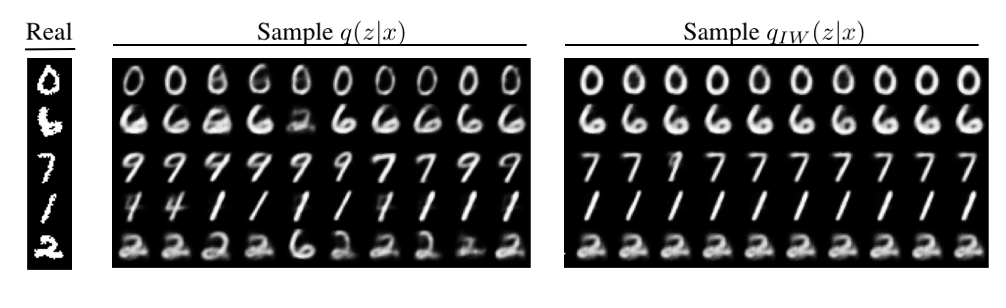
\includegraphics[width=1.\textwidth, clip, trim=0cm .5cm 0cm 0cm]{figs/samps.png}
  \caption{Reconstructions of MNIST samples from $q(z|x)$ and $q_{IW}$.
  The model was trained by maximizing the IWAE ELBO with K=50 and 2 latent dimensions. The reconstructions from $q(z|x)$ are greatly improved with the sampling-resampling step of $q_{IW}$.}
  \label{recon}
\end{figure}

In figure~\ref{recon}, we demonstrate the need to sample from $q_{IW}$ rather than $q(z|x)$ for reconstructing MNIST digits.
We trained the model to maximize the IWAE ELBO with K=50 and 2 latent dimensions, similar to Appendix C in \citet{burda2015importance}.
When we sample from $q(z|x)$ and reconstruct the samples, we see a number of anomalies.
However, if we perform the sampling-resampling step (Alg.~\ref{sampling_qiw}), then the reconstructions are much more accurate.
The intuition here is that we trained the model with $q_{IW}$ with $K=50$ then sampled from $q(z|x)$ ($q_{IW}$ with $K=1$), which are very different distributions, as seen in Fig.~\ref{viz1}.



\section{Discussion}
\cite{bachman} also showed that the IWAE objective is equivalent to stochastic variational inference with a proposal distribution corrected towards the true posterior via normalized importance sampling.
%In other words, the IWAE lower bound can be interpreted as the expectation of the standard VAE lower bound with an implicit $\tilde{q}_{IW}$ distribution which depends on samples.
We build on this idea by further examining $\tilde{q}_{IW}$ and by providing visualizations to help better grasp the interpretation.
To summarize our observations, the following is the ordering of lower bounds given specific proposal distributions,
\begin{align} 
    % log(p(x)) \geq L_{IWAE}[\tilde{q}_{IW}] = L_{VAE}[\tilde{q}_{IW}] \geq L_{IWAE}[q] = L_{VAE}[q_{IW|z\setminus i}] \geq L_{VAE}[q] \nonumber \\
    \log p(x) \geq L_{VAE}[q_{EIW}] \geq \mathbb{E}_{z_{2} \dots z_{k}\sim q(z|x)} \left[ L_{VAE}[\tilde{q}_{IW}(z|z_{2:k})] \right] = L_{IWAE}[q]  \geq L_{VAE}[q] \nonumber
\end{align}
In light of this, IWAE can be seen as increasing the complexity of the approximate distribution $q$, similar to other methods that increase the complexity of $q$, such as Normalizing Flows \citep{normflow}, Variational Boosting \citep{varboosting} or Hamiltonian variational inference \citep{salimans2015markov}.
With this interpretation in mind, we can possibly generalize $\tilde{q}_{IW}$ to be applicable to other divergence measures.
An interesting avenue of future work is the comparison of IW-based variational families with alpha-divergences or operator variational objectives. 









\subsubsection*{Acknowledgments}

We'd like to thank an anonymous ICLR reviewer for providing insightful future directions for this work. We'd also like to thank Yuri Burda, Christian Naesseth, and Scott Linderman for bringing our attention to oversights in the paper. We'd like to thank Christian Naesseth for the derivation in section \ref{qeiw_proof}.

\bibliographystyle{iclr2017_workshop}
\bibliography{iclr2017_workshop}

\newpage

\section{Appendix}

\subsection{Detailed derivation of the equivalence of VAE and IWAE bound}
\label{detailed_derivation}

Here we show that the expectation over $z_2 ... z_k$ of the VAE lower bound with the unnomalized importance weighted distribution $\tilde{q}_{\textnormal{IW}}$, $\mathcal{L}_{\textnormal{VAE}}[\tilde{q}_{\textnormal{IW}}(z|z_{2:k})]$, is equivalent to the IWAE bound with the original $q$ distribution, $\mathcal{L}_{\textnormal{IWAE}}[q]$.

% First, we start by writing the VAE ELBO in its minibatch form, as an average over $k$ samples:
% \begin{align} 
%     \log p(x) &\geq 
%     \mathcal{L}_{VAE}[q] =
%     E_{z \sim q(z|x)} \left[  log\left(\frac{p(x,z)}{q(z|x)} \right) \right]  
%     = E_{z_{1}...z_{k} \sim q(z|x)} \left[  \frac{1}{k}\sum_{i=1}^k log\left(\frac{p(x,z_i)}{q(z|x)} \right) \right]
% \end{align}
% If we now replace $q(z|x)$ with $\tilde{q}_{IW}(z|x,z_{2:k})$, then we recover the IWAE ELBO:
% \begin{align}
%     L_{VAE}[\tilde{q}_{IW}] &= E_{z_{1}...z_{k} \sim \tilde{q}_{IW}(z|x,z_{2:k})} \left[  \frac{1}{k}\sum_{i=1}^k log\left(\frac{p(x,z_i)}{\tilde{q}_{IW}(z_i|x,z_{2:k})}  \right)  \right] \\
%     &= E_{z_{1}...z_{k} \sim \tilde{q}_{IW}(z|x,z_{2:k})} \left[  \frac{1}{k}\sum_{i=1}^k log\left(\frac{p(x,z_i)}{\frac{p(x,z_i)}{\frac{1}{k}   \sum_{j=1}^k \frac{p(x,z_j)}{q(z_j|x)}}}  \right)  \right] \\
%     &= E_{z_{1}...z_{k} \sim \tilde{q}_{IW}(z|x,z_{2:k})} \left[  \frac{1}{k}\sum_{i=1}^k log\left(\frac{1}{k} \sum_{j=1}^k \frac{p(x,z_j)}{q(z_j|x)}\right)  \right] \label{with_i} \\
%     &= E_{z_{1}...z_{k} \sim \tilde{q}_{IW}(z|x,z_{2:k})} \left[ log\left(\frac{1}{k} \sum_{j=1}^k \frac{p(x,z_j)}{q(z_j|x)}\right)  \right]  \label{without_i} \\
%     &= E_{z_{1}...z_{k} \sim q(z|x)} \left[  \sum_{l=1}^k \tilde w_l  \left( log\left(\frac{1}{k} \sum_{j=1}^k \frac{p(x,z_j)}{q(z_j|x)}\right)\right)  \right] \label{with_w} \\ 
%     &= E_{z_{1}...z_{k} \sim q(z|x)} \left[  log\left(\frac{1}{k}\sum_{j=1}^k \frac{p(x,z_j)}{q(z_j|x)}  \right)  \right] = \mathcal{L}_{IWAE}[q] \label{without_w}
% \end{align}
% Eqn. \ref{without_i} follows Eqn. \ref{with_i} since index $i$ is not present within the sum over $i$. At Eqn. \ref{with_w} we use the fact that you can sample $\tilde{q}_{IW}$ by sampling $q$ then summing over the weighted samples. From Eqn. \ref{with_w} to Eqn. \ref{without_w}, index $l$ is not present after $\tilde w_l$ and $\sum_{l=1}^k \tilde w_l$ sums to one. Eqn. \ref{without_w} is the IWAE ELBO, thus we see that VAE with $\tilde{q}_{IW}$ is equivalent to the IWAE ELBO.



% Correct proof:
\begin{align}
    \mathbb{E}_{z_{2} \dots z_{k}\sim q(z|x)} \! \left[ \mathcal{L}_{\textnormal{VAE}}[\tilde{q}_{\textnormal{IW}}(z|z_{2:k})] \right] 
    % &= \mathbb{E}_{z_{2} \dots z_{k} \sim q(z|x)} \!\left[ \mathbb{E}_{z \sim \tilde{q}_{\textnormal{IW}}(z|z_{2:k})} \left[ \log\left(\frac{p(x,z)}{\tilde{q}_{IW}(z|x,z_{2:k})} \right)  \right] \right] \\
    % &= \mathbb{E}_{z_{2} \dots z_{k} \sim q(z|x)} \!\left[ \mathbb{E}_{z \sim \tilde{q}_{\textnormal{IW}}(z|z_{2:k})} \left[ \log\left(\frac{p(x,z)}{\frac{p(x,z)}{\frac{1}{k}   \sum_{i=1}^k \frac{p(x,z_i)}{q(z_i|x)}}} \right)  \right] \right] \\
    % &= \mathbb{E}_{z_{2} \dots z_{k} \sim q(z|x)} \!\left[ \mathbb{E}_{z \sim \tilde{q}_{\textnormal{IW}}(z|z_{2:k})} \left[ \log\left(\frac{1}{k}   \sum_{i=1}^k \frac{p(x,z_i)}{q(z_i|x)} \right)  \right] \right] \\
    &= \mathbb{E}_{z_{2} \dots z_{k} \sim q(z|x)} \!\left[ \int_{z} \tilde{q}_{\textnormal{IW}}(z|x,z_{2:k})  \log\left(\frac{p(x,z)}{\tilde{q}_{IW}(z|x,z_{2:k})} \right)  dz \right] \\
    &= \mathbb{E}_{z_{2} \dots z_{k} \sim q(z|x)} \!\left[ \int_{z} \tilde{q}_{\textnormal{IW}}(z|x,z_{2:k})  \log\left(\frac{p(x,z)}{\frac{p(x,z)}{\frac{1}{k}   \sum_{i=1}^k \frac{p(x,z_i)}{q(z_i|x)}}} \right)  dz \right] \\
    &= \mathbb{E}_{z_{2} \dots z_{k} \sim q(z|x)} \!\left[ \int_{z} \tilde{q}_{\textnormal{IW}}(z|x,z_{2:k}) \log\left(\frac{1}{k}   \sum_{i=1}^k \frac{p(x,z_i)}{q(z_i|x)} \right)  dz \right] \\
    &= \mathbb{E}_{z_{2} \dots z_{k} \sim q(z|x)} \!\left[\int_z  \tilde{q}_{\textnormal{IW}}(z|x,z_{2:k}) \log\left(\frac{1}{k}   \sum_{i=1}^k \frac{p(x,z_i)}{q(z_i|x)} \right)  dz \right]  \\
    % &= \mathbb{E}_{z_{2} \dots z_{k} \sim q(z|x)} \!\left[\int_z  k \tilde{w} q(z|x) \log\left(\frac{1}{k}   \sum_{i=1}^k \frac{p(x,z_i)}{q(z_i|x)} \right)  dz \right]  \\
    % &= \mathbb{E}_{z_{1} \dots z_{k} \sim q(z|x)} \!\left[ k \tilde{w}_1  \log\left(\frac{1}{k}   \sum_{i=1}^k \frac{p(x,z_i)}{q(z_i|x)} \right)   \right]  \label{change_notation}\\
    &= \mathbb{E}_{z_{2} \dots z_{k} \sim q(z|x)} \!\left[\int_z  k \frac{\frac{p(x,z)}{q(z|x)}}{\sum_{j=1}^k \frac{p(x,z_j)}{q(z_j|x)}} q(z|x) \log\left(\frac{1}{k}   \sum_{i=1}^k \frac{p(x,z_i)}{q(z_i|x)} \right)  dz \right]  \\
    &= \mathbb{E}_{z_{2} \dots z_{k} \sim q(z|x)} \!\left[\int_{z_1}  k \frac{\frac{p(x,z_1)}{q(z_1|x)}}{\sum_{j=1}^k \frac{p(x,z_j)}{q(z_j|x)}} q(z|x) \log\left(\frac{1}{k}   \sum_{i=1}^k \frac{p(x,z_i)}{q(z_i|x)} \right)  dz \right] \label{change_notation} \\
    % &= \mathbb{E}_{z_{1} \dots z_{k} \sim q(z|x)} \!\left[ k \frac{\frac{p(x,z_1)}{q(z_1|x)}}{\sum_{j=1}^k \frac{p(x,z_j)}{q(z_j|x)}}  \log\left(\frac{1}{k}   \sum_{i=1}^k \frac{p(x,z_i)}{q(z_i|x)} \right)   \right]  \\
    &= \mathbb{E}_{z_{1} \dots z_{k} \sim q(z|x)} \!\left[ k  \frac{\frac{p(x,z_1)}{q(z_1|x)}}{\sum_{j=1}^k \frac{p(x,z_j)}{q(z_j|x)}}  \log\left(\frac{1}{k}   \sum_{i=1}^k \frac{p(x,z_i)}{q(z_i|x)} \right)   \right]  \\
    &= \mathbb{E}_{z_{1} \dots z_{k} \sim q(z|x)} \left[  \frac{\sum_{j=1}^k \frac{p(x,z_j)}{q(z_j|x)}}{\sum_{j=1}^k \frac{p(x,z_j)}{q(z_j|x)}}  \log\left(\frac{1}{k}   \sum_{i=1}^k \frac{p(x,z_i)}{q(z_i|x)} \right)  \right] \label{sum_k} \\
    &= \mathbb{E}_{z_{1} \dots z_{k} \sim q(z|x)} \left[  \log\left(\frac{1}{k}   \sum_{i=1}^k \frac{p(x,z_i)}{q(z_i|x)} \right)  \right]  \\
    &= \mathcal{L}_{\textnormal{IWAE}}[q] 
  \end{align}


(\ref{change_notation}): Change of notation $z = z_1$.\\
(\ref{sum_k}): $z_i$ has the same expectation as $z_1$ so we can replace $k$ with the sum of $k$ terms.



\newpage





% Thus, when $k=\infty$:
% \begin{align} 
%     \tilde{q}_{IW}(z|x) &= 
%     E_{z_{1}...z_{\infty} \sim q(z|x)} \left[ \frac{p(x,z)}{\lim_{k\to\infty} \frac{1}{k} \sum_{j=1}^k \frac{p(x,z_j)}{q(z_j|x)}} \right] %\textnormal {where $z_1 = z$}
%     = \frac{p(x,z)}{E_{q(z|x)}\left[\frac{p(x,z)}{q(z|x)} \right]}
%     = \frac{p(x,z)}{p(x)} 
%     = p(z|x)
% \end{align}
% Thus $\tilde{q}_{IW}(z)$ is equal to the true posterior $p(z|x)$ when $k=\infty$, as expected.




% \begin{align} 
%     % \tilde{q}_{IW}(z|x) &= E_{z_{1}...z_{k} \sim q(z|x)} \left[ \tilde{q}_{IW}(z|x, z_{\setminus i}) \right] \textnormal{for any $i$}. \\
%     \tilde{q}_{IW}(z|x) &= E_{z_{2}...z_{k} \sim q(\cdot |x)} \left[ \frac{p(x)}{  \frac{1}{k} \left( \frac{p(x,z)}{q(z|x)}+ \sum_{j=2}^k \frac{p(x,z_j)}{q(z_j|x)} \right) } \right] p(z|x) %\label{marg} %\textnormal {where $z_1 = z$}. 
% \end{align}







\subsection{Proof that \texorpdfstring{$q_{EIW}$}{} is a normalized distribution}
\label{proof_norm}

\begin{align} 
    \int_z q_{EIW}(z|x) dz
    &= \int_z E_{z_{2}...z_{k} \sim q(z|x)} \left[ \tilde{q}_{IW}(z|x,z_{2:k}) \right] dz \\
    &= \int_z E_{z_{2}...z_{k} \sim q(z|x)} \left[ \frac{p(x,z)}{  \frac{1}{k} \left( \frac{p(x,z)}{q(z|x)}+ \sum_{j=2}^k \frac{p(x,z_j)}{q(z_j|x)} \right) } \right] dz\\
    &= \int_z \frac{q(z|x)}{q(z|x)}E_{z_{2}...z_{k} \sim q(z|x)} \left[ \frac{p(x,z)}{  \frac{1}{k} \left( \frac{p(x,z)}{q(z|x)}+ \sum_{j=2}^k \frac{p(x,z_j)}{q(z_j|x)} \right) } \right] dz\\
    &= E_{z \sim q(z|x)} E_{z_{2}...z_{k} \sim q(z|x)} \left[ \frac{\frac{p(x,z)}{q(z|x)}}{  \frac{1}{k} \left( \frac{p(x,z)}{q(z|x)}+ \sum_{j=2}^k \frac{p(x,z_j)}{q(z_j|x)} \right) } \right] \\
    &= E_{z_{1}...z_{k} \sim q(z|x)} \left[ \frac{\frac{p(x,z_1)}{q(z_1|x)}}{  \frac{1}{k} \left( \sum_{j=1}^k \frac{p(x,z_j)}{q(z_j|x)} \right) } \right] \label{nota} \\
    &= k*E_{z_{1}...z_{k} \sim q(z|x)} \left[ \frac{\frac{p(x,z_1)}{q(z_1|x)}}{   \sum_{j=1}^k \frac{p(x,z_j)}{q(z_j|x)}  } \right]\\
    &= \sum_{i=1}^{k} E_{z_{1}...z_{k} \sim q(z|x)} \left[ \frac{\frac{p(x,z_i)}{q(z_i|x)}}{   \sum_{j=1}^k \frac{p(x,z_j)}{q(z_j|x)}  } \right] \label{to_sum} \\
    &= E_{z_{1}...z_{k} \sim q(z|x)} \left[ \frac{\sum_{i=1}^k \frac{p(x,z_i)}{q(z_i|x)}}{   \sum_{j=1}^k \frac{p(x,z_j)}{q(z_j|x)}  } \right] \label{linear} \\
    &= E_{z_{1}...z_{k} \sim q(z|x)} \left[1 \right] \\
    &= 1
\end{align}


(\ref{nota}): Change of notation $z = z_1$. \\
(\ref{to_sum}): $z_i$ has the same expectation as $z_1$ so we can replace $k$ with the sum of $k$ terms. \\
(\ref{linear}): Linearity of expectation.

\newpage

\subsection{Proof that \texorpdfstring{$\mathcal{L}_{VAE}[q_{EIW}]$}{} is an upper bound of \texorpdfstring{$\mathcal{L}_{IWAE}[q]$}{}}
\label{qeiw_proof}

Proof provided by Christian Naesseth.
% Previous proof

% \begin{align} 
%     \mathcal{L}_{VAE}[q_{EIW}] &= E_{z \sim q_{EIW}} \left[ log \left( \frac{p(x,z)}{q_{EIW}(z|x)} \right) \right] \\
%     &= E_{z \sim q_{EIW}} \left[ log(p(x,z)) - log \left( E_{z_{2}...z_{k} \sim q(\cdot |x)} \left[ \frac{p(x,z)}{  \frac{1}{k} \left( \frac{p(x,z)}{q(z|x)}+ \sum_{j=2}^k \frac{p(x,z_j)}{q(z_j|x)} \right) } \right] \right) \right] \\
%     &= E_{z \sim q_{EIW}} \left[ - log \left( E_{z_{2}...z_{k} \sim q(\cdot |x)} \left[ \frac{1}{  \frac{1}{k} \left( \frac{p(x,z)}{q(z|x)}+ \sum_{j=2}^k \frac{p(x,z_j)}{q(z_j|x)} \right) } \right] \right) \right] \\
%     &= E_{z \sim q_{EIW}} \left[log \left( E_{z_{2}...z_{k} \sim q(\cdot |x)} \left[  \frac{1}{k} \left( \frac{p(x,z)}{q(z|x)}+ \sum_{j=2}^k \frac{p(x,z_j)}{q(z_j|x)} \right)  \right] \right) \right] \\
%     & \geq E_{z \sim q_{EIW}} \left[E_{z_{2}...z_{k} \sim q(\cdot |x)} \left[ log \left(   \frac{1}{k} \left( \frac{p(x,z)}{q(z|x)}+ \sum_{j=2}^k \frac{p(x,z_j)}{q(z_j|x)} \right)   \right) \right] \right] \\
%     &= E_{z_{1}...z_{k} \sim q(\cdot |x)} \left[ log \left(   \frac{1}{k} \left( \frac{p(x,z_{1})}{q(z_{1}|x)}+ \sum_{j=2}^k \frac{p(x,z_j)}{q(z_j|x)} \right)   \right) \right]\\
%     &= \mathcal{L}_{IWAE}[q] 
% \end{align}


Let $\hat{p}(x|z_{1:k})=\frac{1}{k} \left( \frac{p(x,z)}{q(z|x)}+ \sum_{j=2}^k \frac{p(x,z_j)}{q(z_j|x)} \right)$
\begin{align} 
    \mathcal{L}_{VAE}[q_{EIW}] &= E_{z \sim q_{EIW}} \left[ log \left( \frac{p(x,z)}{q_{EIW}(z|x)} \right) \right] \\
    &= E_{z \sim q_{EIW}} \left[ log \left( \frac{p(x,z)}{E_{q(z_{2:k} |x)} \left[ \frac{p(x,z)}{ \hat{p}(x|z_{1:k})} \right]}  \right) \right] \\
    &= E_{z \sim q_{EIW}} \left[ log \left( \frac{1}{E_{q(z_{2:k} |x)} \left[ \frac{1}{ \hat{p}(x|z_{1:k}) } \right]}  \right) \right] \\
    &= E_{z \sim q_{EIW}} \left[ - log \left( E_{q(z_{2:k} |x)} \left[  \hat{p}(x|z_{1:k})^{-1} \right] \right) \right] \\   
    &= - \int_{z} p(x,z) E_{q(z_{2:k} |x)} \left[  \hat{p}(x|z_{1:k})^{-1} \right] log \left( E_{q(z_{2:k} |x)} \left[  \hat{p}(x|z_{1:k})^{-1} \right] \right) dz \\  
    &\geq - \int_{z} p(x,z) E_{q(z_{2:k} |x)} \left[  \hat{p}(x|z_{1:k})^{-1} log \left(  \hat{p}(x|z_{1:k})^{-1} \right) \right]  dz \label{geq} \\   
    &= - \int_{z} p(x,z) \int_{z_{2:k}} q(z_{2:k} |x) \hat{p}(x|z_{1:k})^{-1} log \left(  \hat{p}(x|z_{1:k})^{-1} \right)  dz \\  
    &= - \int_{z_{1:k}}  \frac{q(z_1|x)}{q(z_1|x)} p(x,z_1)  q(z_{2:k} |x)  \hat{p}(x|z_{1:k})^{-1} log \left(  \hat{p}(x|z_{1:k})^{-1} \right)   dz \label{z1} \\ 
    &= - \int_{z_{1:k}}  \frac{p(x,z_1)}{q(z_1|x)}   q(z_{1:k} |x)  \hat{p}(x|z_{1:k})^{-1} log \left(  \hat{p}(x|z_{1:k})^{-1} \right)   dz \\ 
    &= \int_{z_{1:k}}  \frac{\frac{p(x,z_1)}{q(z_1|x)}}{\hat{p}(x|z_{1:k})}     q(z_{1:k} |x)  log \left(  \hat{p}(x|z_{1:k}) \right)   dz \\ 
    &= k \int_{z_{1:k}}  \frac{\frac{p(x,z_1)}{q(z_1|x)}}{ \sum_{j=1}^k \frac{p(x,z_j)}{q(z_j|x)} }     q(z_{1:k} |x)  log \left(  \frac{1}{k} \sum_{j=1}^k \frac{p(x,z_j)}{q(z_j|x)} \right)   dz \\ 
    &= \sum_{i=1}^{k} \int_{z_{1:k}}  \frac{\frac{p(x,z_i)}{q(z_i|x)}}{ \sum_{j=1}^k \frac{p(x,z_j)}{q(z_j|x)} }     q(z_{1:k} |x)  log \left(  \frac{1}{k} \sum_{j=1}^k \frac{p(x,z_j)}{q(z_j|x)} \right)   dz \label{sum} \\ 
    &=  \int_{z_{1:k}}  \frac{ \sum_{i=1}^{k} \frac{p(x,z_i)}{q(z_i|x)}}{ \sum_{j=1}^k \frac{p(x,z_j)}{q(z_j|x)} }     q(z_{1:k} |x)  log \left(  \frac{1}{k} \sum_{j=1}^k \frac{p(x,z_j)}{q(z_j|x)} \right)   dz \\
    &=  \int_{z_{1:k}} q(z_{1:k} |x)  log \left(  \frac{1}{k} \sum_{j=1}^k \frac{p(x,z_j)}{q(z_j|x)} \right)   dz \\
    &= E_{q(z_{1:k})} \left[ log \left(  \frac{1}{k} \sum_{j=1}^k \frac{p(x,z_j)}{q(z_j|x)} \right)  \right] \\
    &= \mathcal{L}_{IWAE}[q] 
\end{align}

(\ref{geq}): Given that $f(A)=-AlogA$ is concave for $A>0$, and $f(E[x])\geq E[f(x)]$, then $f(E[x])=-E[x]logE[x]\geq E[-xlogx]$.\\ 
(\ref{z1}): Change of notation $z = z_1$.\\
(\ref{sum}): $z_i$ has the same expectation as $z_1$ so we can replace $k$ with the sum of $k$ terms.



% \subsection{Proof that \texorpdfstring{$\mathcal{L}_{VAE}[q_{EIW}]$}{} is an upper bound of \texorpdfstring{$\mathcal{L}_{VAE}[q]$}{}}


% \begin{align} 
%     \mathcal{L}_{VAE}[q] &= E_{z_{1}...z_{k} \sim q} \left[ \frac{1}{k} \sum^{k} log \left( \frac{p(x,z)}{q(z|x)} \right) \right] \\
%     &= E_{z_{1}} \left[ E_{z_{2}...z_{k} \sim q} \left[ \frac{1}{k} \sum^{k} log \left( \frac{p(x,z)}{q(z|x)} \right) \right] \right] \\
%     &\leq E_{z_{1}} \left[ E_{z_{2}...z_{k} \sim q} \left[ log \frac{1}{k} \sum^{k} \left( \frac{p(x,z)}{q(z|x)} \right) \right] \right] \\
%     &\leq E_{z_{1}} \left[ log E_{z_{2}...z_{k} \sim q} \left[  \frac{1}{k} \sum^{k} \left( \frac{p(x,z)}{q(z|x)} \right) \right] \right] \\
%     &= E_{z_{1}} \left[ -log \frac{1}{E_{z_{2}...z_{k} \sim q} \left[  \frac{1}{k} \sum^{k} \left( \frac{p(x,z)}{q(z|x)} \right) \right]}  \right] \\
%     &= E_{z_{1}} \left[ -log \frac{1}{E_{z_{2}...z_{k} \sim q} \left[  A \right]}  \right] \\
%     % &= E_{z \sim q_{EIW}} \left[ log \left( \frac{p(x,z)}{E_{z_{2}...z_{k} \sim q(\cdot |x)} \left[ \frac{p(x,z)}{ A } \right]}  \right) \right] \\
%     % &= E_{z \sim q_{EIW}} \left[ log \left( \frac{1}{E_{z_{2}...z_{k} \sim q(\cdot |x)} \left[ \frac{1}{ A } \right]}  \right) \right] \\
%     % &= E_{z \sim q_{EIW}} \left[ - log \left( E_{z_{2}...z_{k} \sim q(\cdot |x)} \left[ \frac{1}{  A } \right] \right) \right] \\
%     % % &= E_{z \sim q_{EIW}} \left[log \left( E_{z_{2}...z_{k} \sim q(\cdot |x)} \left[  A  \right] \right) \right] \\
%     % & \leq E_{z \sim q_{EIW}} \left[-E_{z_{2}...z_{k} \sim q(\cdot |x)} \left[ log \left(   \frac{1}{A}   \right) \right] \right] \\
%     % &= E_{z \sim q_{EIW}} \left[E_{z_{2}...z_{k} \sim q(\cdot |x)} \left[ log \left( A   \right) \right] \right] \\
%     % &= E_{z_{1}...z_{k} \sim q(\cdot |x)} \left[ log \left(   A   \right) \right]\\
%     % &= \mathcal{L}_{IWAE}[q] 
% \end{align}



% \begin{align} 
%     \mathcal{L}_{VAE}[q] &= E_{z_{1}...z_{k} \sim q} \left[ \frac{1}{k} \sum^{k} log \left( \frac{p(x,z)}{q(z|x)} \right) \right] \\
%     &= E_{z_{1}} \left[ E_{z_{2}...z_{k} \sim q} \left[ \frac{1}{k} \sum^{k} log \left( \frac{p(x,z)}{q(z|x)} \right) \right] \right] \\
%     &\leq E_{z_{1}} \left[ E_{z_{2}...z_{k} \sim q} \left[ log A \right] \right] \\
%     &= E_{z_{1}} \left[ E_{z_{2}...z_{k} \sim q} \left[ -log \frac{1}{A} \right] \right] \\
%     &\geq E_{z_{1}} \left[ -log E_{z_{2}...z_{k} \sim q} \left[  \frac{1}{A} \right] \right] \\
%     &= L_{VAE}[q_{EIW}]
%     % &\leq E_{z_{1}} \left[ log E_{z_{2}...z_{k} \sim q} \left[  A \right] \right] \\
%     % &= E_{z_{1}} \left[ -log \frac{1}{E_{z_{2}...z_{k} \sim q} \left[  A \right]}  \right] 
% \end{align}



\subsection{Proof that \texorpdfstring{$q_{EIW}$}{} is closer to the true posterior than \texorpdfstring{$q$}{}}

% Section \ref{detailed_derivation}
The previous section showed that $\mathcal{L}_{IWAE}(q) \leq \mathcal{L}_{VAE}(q_{EIW})$. That is, the IWAE ELBO with the base $q$ is a lower bound to the VAE ELBO with the importance weighted $q_{EIW}$. Due to Jensen\textquotesingle s inequality and as shown in \cite{burda2015importance}, we know that the IWAE ELBO is an upper bound of the VAE ELBO: ${L}_{IWAE}(q) \geq {L}_{VAE}(q)$. Furthermore, the log marginal likelihood can be factorized into: $log(p(x)) = {L}_{VAE}(q) + KL(q||p)$, and rearranged to: $KL(q||p) = log(p(x)) - {L}_{VAE}(q)$.

Following the observations above and substituting $q_{EIW}$ for $q$:
\begin{align} 
    KL(q_{EIW}||p) &= log(p(x)) - {L}_{VAE}[q_{EIW}] \\
    &\leq log(p(x)) - {L}_{IWAE}[q] \\
    &\leq log(p(x)) - {L}_{VAE}[q] = KL(q||p)
\end{align}
Thus, $KL(q_{EIW}||p) \leq KL(q||p)$, meaning $q_{EIW}$ is closer to the true posterior than $q$ in terms of KL divergence. 

\subsection{In the limit of the number of samples}

Another perspective is in the limit of ${k=\infty}$. Recall that the marginal likelihood can be approximated by importance sampling:
\begin{align} 
    p(x) &= E_{q(z|x)}\left[\frac{p(x,z)}{q(z|x)} \right] \approx \frac{1}{k}\sum_i^k \frac{p(x,z_i)}{q(z_i|x)}
\end{align}
where $z_i$ is sampled from $q(z_i|x)$. We see that the denominator of $\tilde{q}_{IW}$ is approximating $p(x)$. If $\frac{p(x,z)}{q(z|x)}$ is bounded, then it follows from the strong law of large numbers that, as $k$ approaches infinity, $\tilde{q}_{IW}$ converges to the true posterior $p(z|x)$ almost surely. This interpretation becomes clearer when we factor out the true posterior from $\tilde{q}_{IW}$:
\begin{align} 
\tilde{q}_{IW}(z|x,z_{2:k}) =  \frac{p(x)}{  \frac{1}{k} \left( \frac{p(x,z)}{q(z|x)}+ \sum_{j=2}^k \frac{p(x,z_j)}{q(z_j|x)} \right) }  p(z|x)
\end{align}
We see that the closer the denominator becomes to $p(x)$, the closer $\tilde{q}_{IW}$ is to the true posterior.








\subsection{Visualizing \texorpdfstring{$\tilde{q}_{IW}$}{} in 1D}
\label{viz_section}

\begin{figure}[H]
  \centering
      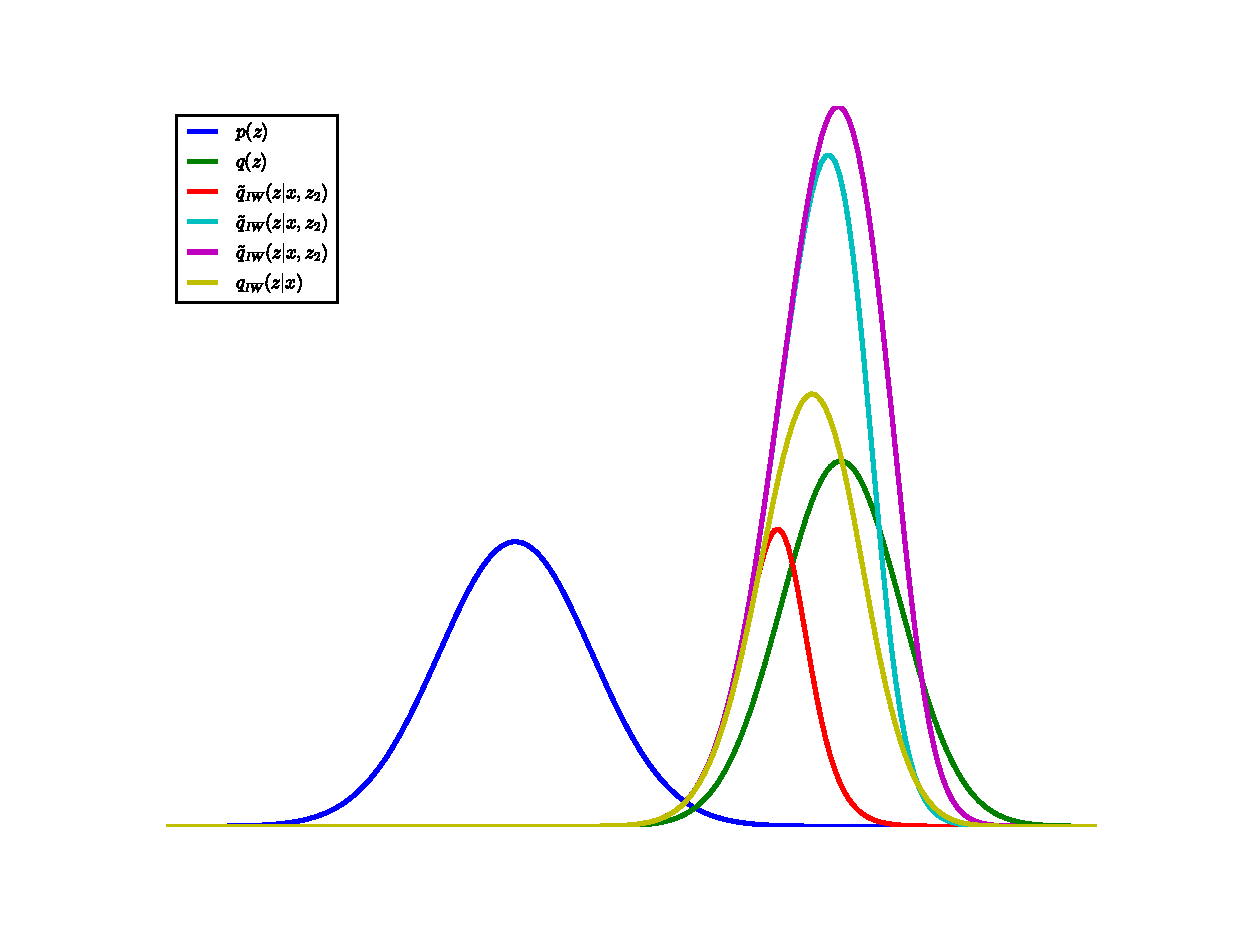
\includegraphics[width=.5\textwidth]{figs/figure_1.eps}
  \caption{Visualization of three 1D $\tilde{q}_{IW}$ distributions. The blue $p(z)$ distribution and the green $q(z)$ distribution are both normalized. The other three distributions are instances of $\tilde{q}_{IW}(z|z_2)$ ($k=2$) with different $z_2$ samples from $q(z)$ and we can see that they are unnormalized. The $\tilde{q}_{IW}$ distributions were plotted using Algorithm \ref{plotting_qeiw} with $S=1$.}
  \label{viz}
\end{figure}




% \section{Visualizing \texorpdfstring{$q_{EIW}$}{} in 1D}

% We can look at the intermediate variational distributions with different numbers of samples $k$ in 1 dimension. Fig. \ref{viz} demonstrates how the approximate posterior approaches the true posterior as $k$ increases. 

% \begin{figure}[H]
%   \centering
%       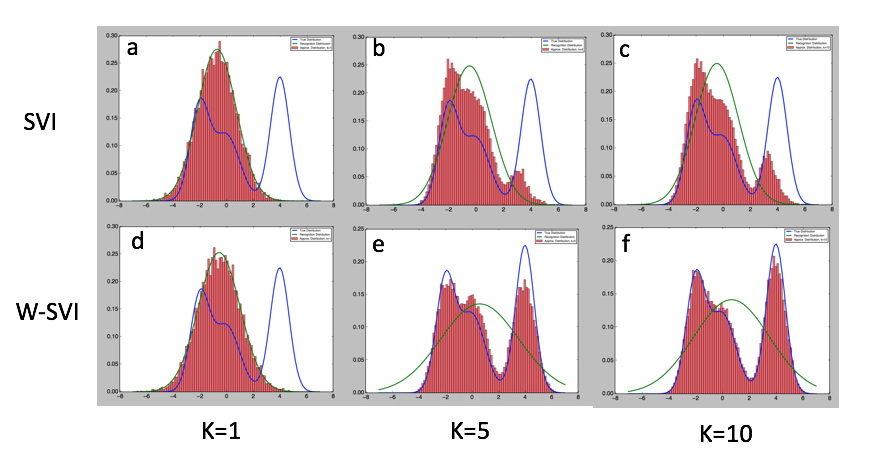
\includegraphics[width=1.\textwidth]{figs/posteriors.png}
%   \caption{Visualization of the importance weighted posterior. The blue distribution is the intractable distribution that we are trying to approximate. The green distribution is the variational distribution. The variational distributions of a, b, and c were optimized via SVI, whereas d, e, and f were optimized with SVI with the IWAE ELBO. The red histograms are importance weighted samples from the variational distribution.}
%   \label{viz}
% \end{figure}





% \section{new stuff}


% \begin{figure*}[h]
% \centering
% \begin{centering}
% \begin{minipage}[t]{0.49\columnwidth}
% \begin{algorithm}[H]
% \caption{Plotting $\tilde{q}_{IW}(z|z_2...z_k)$}\label{plotting_qiw}
% \begin{algorithmic}[1]
%     \State $\textit{k} \gets \textit{number of samples}$
%     \State $z_2\dots z_k \sim q(z)$
%     % \Function{$\tilde{q}_{IW}$}{$z_1, z_2...z_k$}
%     %     \State return $\frac{p(x,z_1)}{\frac{1}{k} \left(  \frac{p(x,z_1)}{q(z_1|x)}+ \sum_{j=2}^k \frac{p(x,z_j)}{q(z_j|x)} \right)}$
%     % \EndFunction
%     \State $A=\sum_{i=2}^{k} \frac{p(z_i)}{q(z_i)}$
%     % \For {$i$ in $1 \dots k$}
%     %     \State $w_i = \frac{p(z_i)}{q(z_i)}$
%     % \EndFor    
%     % \State Each $\tilde w = w_i/\sum_{i=1}^{k} w_i$
%     % \State $j \sim Cat(\tilde{w})$
%     \For {$z$ in plotting space}
%         \State $\tilde{q}_{IW}(z|z_2...z_k) = \frac{p(x,z)}{\frac{1}{k} \left(  \frac{p(x,z)}{q(z|x)}+ A \right)}$
%     \EndFor
%     % \State Return $z_j$
% \end{algorithmic}
% \end{algorithm}
% \end{minipage}
% \end{centering}

% \hfill
% \caption{Procedure to plot $\tilde{q}_{IW}$.}
% \end{figure*}






% \begin{figure}[H]
%   \centering
%       \subfloat[Plotting]
%         {
%             \begin{minipage}[t]{0.43\columnwidth}
%             \begin{algorithm}[H]
%             \caption{Plotting $\tilde{q}_{IW}(z|z_2...z_k)$}\label{plotting_qiw}
%             \begin{algorithmic}[1]
%                 \State $\textit{k} \gets \textit{number of samples}$
%                 \State $z_2\dots z_k \sim q(z)$
%                 \State $A=\sum_{i=2}^{k} \frac{p(z_i)}{q(z_i)}$
%                 \For {$z$ in plotting space}
%                     \State $\tilde{q}_{IW}(z|z_2...z_k) = \frac{p(x,z)}{\frac{1}{k} \left(  \frac{p(x,z)}{q(z|x)}+ A \right)}$
%                 \EndFor
%             \end{algorithmic}
%             \end{algorithm}
%             \end{minipage}
%         }
%       \qquad \qquad %\hfill
%       \subfloat[Sampling]
%         {
%             \begin{minipage}[t]{0.43\columnwidth}
%             \begin{algorithm}[H]
%             \caption{Sampling $\tilde{q}_{IW}(z|z_2...z_k)$}\label{sampling_qiw}
%             \begin{algorithmic}[1]
%                 \State $\textit{k} \gets \textit{number of samples}$
%                 \State $z_2\dots z_k \sim q(z)$
%                 \State $w_i = \frac{p(x,z_i)}{q(z_i|x)}$
%                 \State $\tilde w_i = w_i/\sum_{i=1}^{k} w_i$
%                 \State $j \sim Categorical(\tilde{w})$
%                 \State Return $z_j$
%             \end{algorithmic}
%             \end{algorithm}
%             \end{minipage}
%         }
%       \caption{Probabilistic graphical model of a auxiliary variable model}
%       \label{figure6}
% \end{figure}



% \begin{figure}[H]
%   \centering
%       \subfloat[Plotting]
%         {
%             \begin{minipage}[t]{0.43\columnwidth}
%             \begin{algorithm}[H]
%             \caption{Plotting $\tilde{q}_{IW}(z|z_2...z_k)$}\label{plotting_qiw}
%             \begin{algorithmic}[1]
%                 \State $\textit{k} \gets \textit{number of samples}$
%                 \State $z_2\dots z_k \sim q(z)$
%                 \State $A=\sum_{i=2}^{k} \frac{p(z_i)}{q(z_i)}$
%                 \For {$z$ in plotting space}
%                     \State $\tilde{q}_{IW}(z|z_2...z_k) = \frac{p(x,z)}{\frac{1}{k} \left(  \frac{p(x,z)}{q(z|x)}+ A \right)}$
%                 \EndFor
%             \end{algorithmic}
%             \end{algorithm}
%             \end{minipage}
%         }
%       \qquad \qquad %\hfill
%       \subfloat[Sampling]
%         {
%             \begin{minipage}[t]{0.43\columnwidth}
%             \begin{algorithm}[H]
%             \caption{Sampling $\tilde{q}_{IW}(z|z_2...z_k)$}\label{sampling_qiw}
%             \begin{algorithmic}[1]
%                 \State $\textit{k} \gets \textit{number of samples}$
%                 \State $z_2\dots z_k \sim q(z)$
%                 \State $w_i = \frac{p(x,z_i)}{q(z_i|x)}$
%                 \State $\tilde w_i = w_i/\sum_{i=1}^{k} w_i$
%                 \State $j \sim Categorical(\tilde{w})$
%                 \State Return $z_j$
%             \end{algorithmic}
%             \end{algorithm}
%             \end{minipage}
%         }
%       \caption{Probabilistic graphical model of a auxiliary variable model}
%       \label{figure6}
% \end{figure}



% \begin{figure}[H]
%   \centering
%       \subfloat[Plotting]
%         {
%             \begin{minipage}[t]{0.43\columnwidth}
%             \begin{algorithm}[H]
%             \caption{Plotting $q_{EIW}(z)$}\label{plotting_qeiw}
%             \begin{algorithmic}[1]
%                 \State $\textit{k} \gets \textit{number of samples}$
%                 \State $z_2\dots z_k \sim q(z)$
%                 \State $A=\sum_{i=2}^{k} \frac{p(z_i)}{q(z_i)}$
%                 \For {$z$ in plotting space}
%                     \State $\tilde{q}_{IW}(z|z_2...z_k) = \frac{p(x,z)}{\frac{1}{k} \left(  \frac{p(x,z)}{q(z|x)}+ A \right)}$
%                 \EndFor
%             \end{algorithmic}
%             \end{algorithm}
%             \end{minipage}
%         }
%       \qquad \qquad %\hfill
%       \subfloat[Sampling]
%         {
%             \begin{minipage}[t]{0.43\columnwidth}
%             \begin{algorithm}[H]
%             \caption{Sampling $q_{EIW}(z)$}\label{sampling_qeiw}
%             \begin{algorithmic}[1]
%                 \State $\textit{k} \gets \textit{number of samples}$
%                 \State $z_2\dots z_k \sim q(z)$
%                 \State $w_i = \frac{p(x,z_i)}{q(z_i|x)}$
%                 \State $\tilde w_i = w_i/\sum_{i=1}^{k} w_i$
%                 \State $j \sim Categorical(\tilde{w})$
%                 \State Return $z_j$
%             \end{algorithmic}
%             \end{algorithm}
%             \end{minipage}
%         }
%       \caption{Probabilistic graphical model of a auxiliary variable model}
%       \label{figure_this}
% \end{figure}



  
  
  
  
  
  
%  \section{Visualizing \texorpdfstring{$\tilde{q}_{IW}$}{} in 1D}
  

% \begin{figure}[H]
%   \centering
%       \subfloat[Plotting]
%         {
%             \begin{minipage}[t]{0.43\columnwidth}
%             \begin{algorithm}[H]
%             \caption{Plotting $\tilde{q}_{IW}(z|z_2...z_k)$}\label{plotting_qiw}
%             \begin{algorithmic}[1]
%                 \State $\textit{k} \gets \textit{number of samples}$
%                 \State $z_2\dots z_k \sim q(z)$
%                 \State $A=\sum_{i=2}^{k} \frac{p(z_i)}{q(z_i)}$
%                 \For {$z$ in plotting space}
%                     \State $\tilde{q}_{IW}(z|z_2...z_k) = \frac{p(x,z)}{\frac{1}{k} \left(  \frac{p(x,z)}{q(z|x)}+ A \right)}$
%                 \EndFor
%             \end{algorithmic}
%             \end{algorithm}
%             \end{minipage}
%         }
%       \qquad \qquad %\hfill
%       \subfloat[Sampling]
%         {
%             \begin{minipage}[t]{0.43\columnwidth}
%             \begin{algorithm}[H]
%             \caption{Sampling $\tilde{q}_{IW}(z|z_2...z_k)$}\label{sampling_qiw}
%             \begin{algorithmic}[1]
%                 \State $\textit{k} \gets \textit{number of samples}$
%                 \State $z_2\dots z_k \sim q(z)$
%                 \State $w_i = \frac{p(x,z_i)}{q(z_i|x)}$
%                 \State $\tilde w_i = w_i/\sum_{i=1}^{k} w_i$
%                 \State $j \sim Categorical(\tilde{w})$
%                 \State Return $z_j$
%             \end{algorithmic}
%             \end{algorithm}
%             \end{minipage}
%         }
%       \caption{Probabilistic graphical model of a auxiliary variable model}
% \end{figure}
  



\end{document}

